\documentclass[aspectratio=169]{beamer}
\usetheme{Madrid}
\usecolortheme{whale}
\usepackage[utf8]{inputenc}
\usepackage{graphicx}
\usepackage{amsmath}

\title{Fundamentos de Inteligencia Artificial}
\subtitle{Machine Learning y la Jerarquía de Datos}
\author{Clase Guiada - Semana 1}
\date{}

\begin{document}

\begin{frame}
    \titlepage
\end{frame}

\begin{frame}{Dominios de la Inteligencia Artificial}
    \begin{itemize}
        \item \textbf{Inteligencia Artificial (IA):} El superconjunto. Sistemas que simulan el razonamiento humano. (Ej. Reglas fijas, si A entonces B).
        \item \textbf{Machine Learning (ML):} Algoritmos que aprenden patrones directamente de los datos, sin programación explícita.
        \item \textbf{Deep Learning (DL):} Subcampo del ML. Usa Redes Neuronales Artificiales multicapa para datos no estructurados complejos (Imágenes, Audio).
    \end{itemize}
\end{frame}

\begin{frame}{La Analogía del Parque de Diversiones}
    \begin{columns}
        \column{0.5\textwidth}
        \textbf{El Robot (IA Clásica)} \\
        Tiene un manual estricto. "Si ves rojo, salta". No aprende.
        \vspace{0.5cm}
        
        \textbf{El Cachorro (Machine Learning)} \\
        Aprende por recompensas y ejemplos repetitivos. Encuentra sus propios patrones.
        
        \column{0.5\textwidth}
        \textbf{El Detective (Deep Learning)} \\
        Usa supergafas para ver millones de hilos invisibles y reconstruir imágenes súper complejas.
    \end{columns}
\end{frame}

\begin{frame}{Formalización Matemática: El Vector de Características}
    Cada muestra del mundo real (ej. un paquete de red, un pixel) se transforma en un vector matemático:
    
    \begin{block}{Feature Vector}
    $$\mathbf{x}_i = [x_{i,1}, x_{i,2}, \dots, x_{i,d}]^T \in \mathbb{R}^d$$
    \end{block}
    
    \begin{itemize}
        \item $\mathbf{x}_i$ representa la $i$-ésima muestra.
        \item $d$ representa la dimensionalidad (cantidad de columnas o features).
        \item $x_{i,j}$ es el valor numérico de la característica $j$.
    \end{itemize}
\end{frame}

\begin{frame}{La Función de Mapeo Predictivo}
    El objetivo del aprendizaje supervisado es aproximar una función predictiva $f$:
    
    \begin{block}{Target Function}
    $$f: \mathcal{X} \to \mathcal{Y}$$
    \end{block}
    
    \textbf{Clasificación Binaria} (Malware vs Legítimo):
    $$\mathcal{Y} = \{0, 1\}$$
    
    \textbf{Regresión} (Tiempo de renderizado):
    $$\mathcal{Y} = \mathbb{R}$$
\end{frame}

\begin{frame}{La Jerarquía de Necesidades de Datos (Monica Rogati)}
    No podemos crear modelos avanzados sin cimientos robustos:
    \begin{center}
        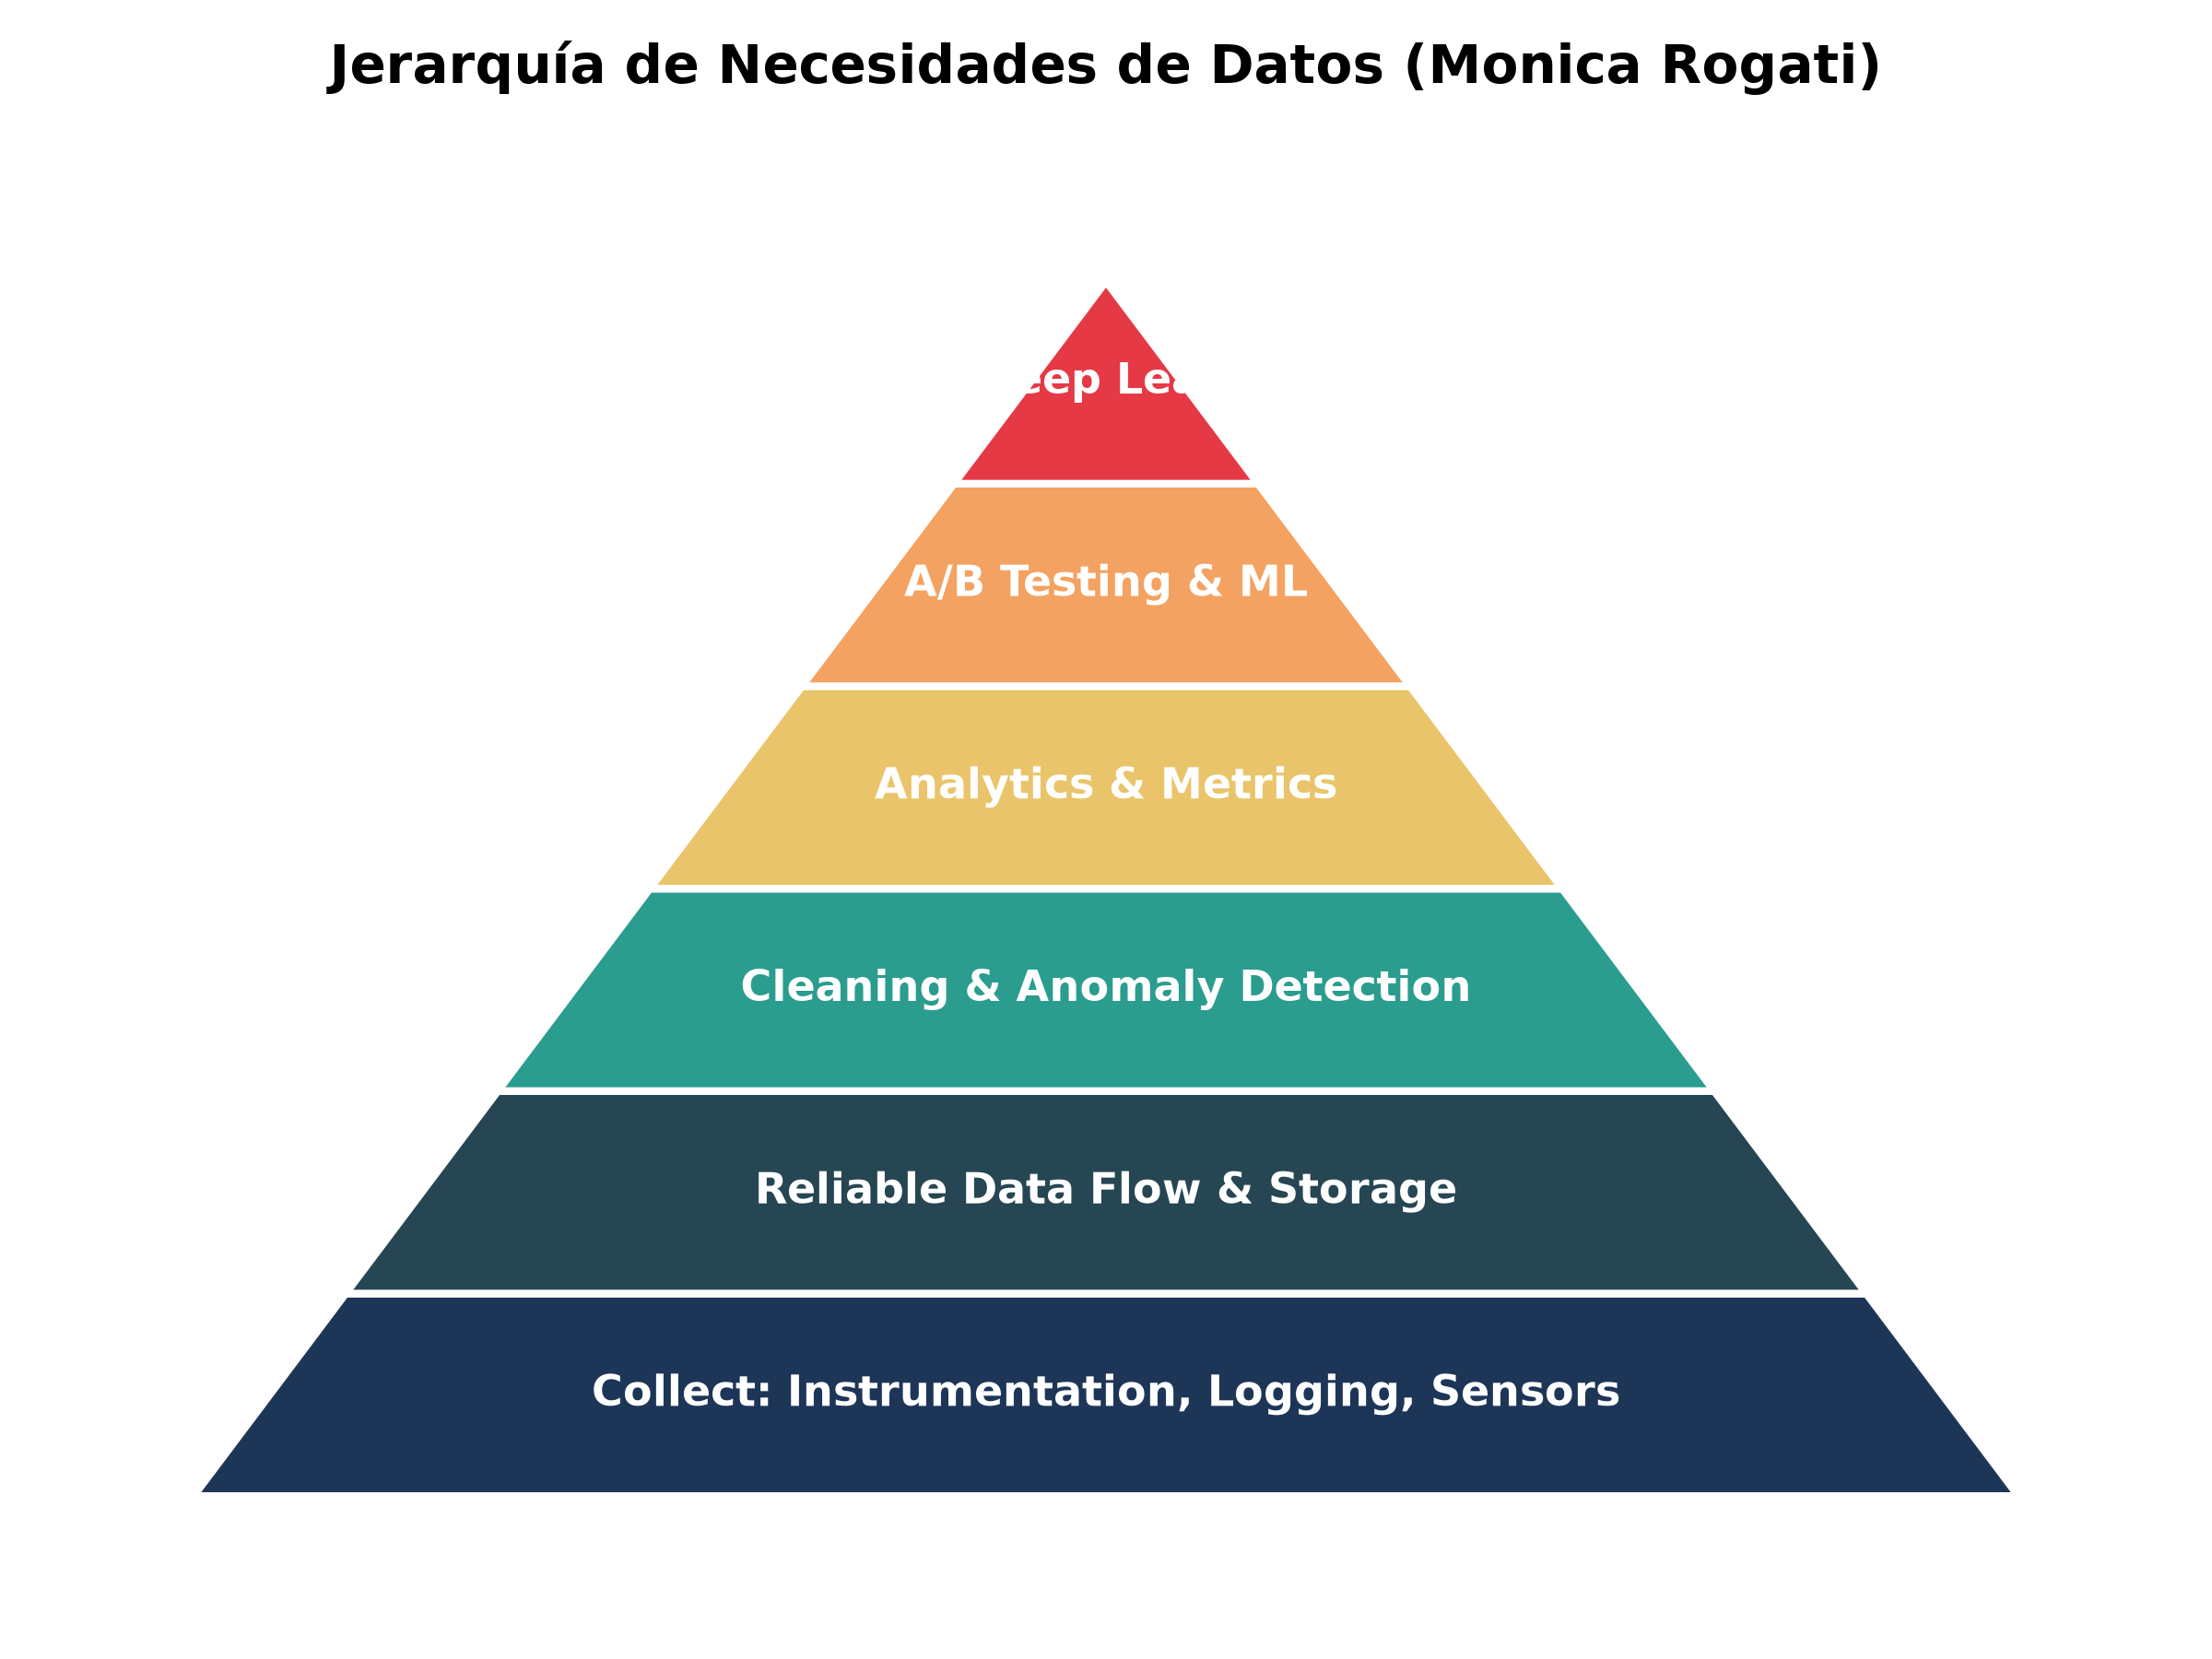
\includegraphics[width=0.55\textwidth]{jerarquia_datos.png}
    \end{center}
    El 80\% del trabajo es recolección y limpieza de datos (Pandas).
\end{frame}

\begin{frame}{Métricas de Desempeño: Tiro al Blanco}
    En Ciberseguridad, un error cuesta millones:
    \begin{itemize}
        \item \textbf{Falso Positivo (Fricción):} El modelo cree que el renderizado 3D es malware y bloquea el acceso. Pérdida de tiempo.
        \item \textbf{Falso Negativo (Brecha):} El modelo deja pasar el Ransomware creyendo que es inofensivo. \textbf{Catástrofe.}
    \end{itemize}
    \vspace{0.5cm}
    Buscamos un modelo con altísima \textbf{Sensibilidad (Recall)} para no dejar escapar ninguna amenaza.
\end{frame}

\begin{frame}{Fin de la Teoría}
    \begin{center}
        \Large ¡Pasemos a la Práctica con Pandas!
    \end{center}
\end{frame}

\end{document}
